
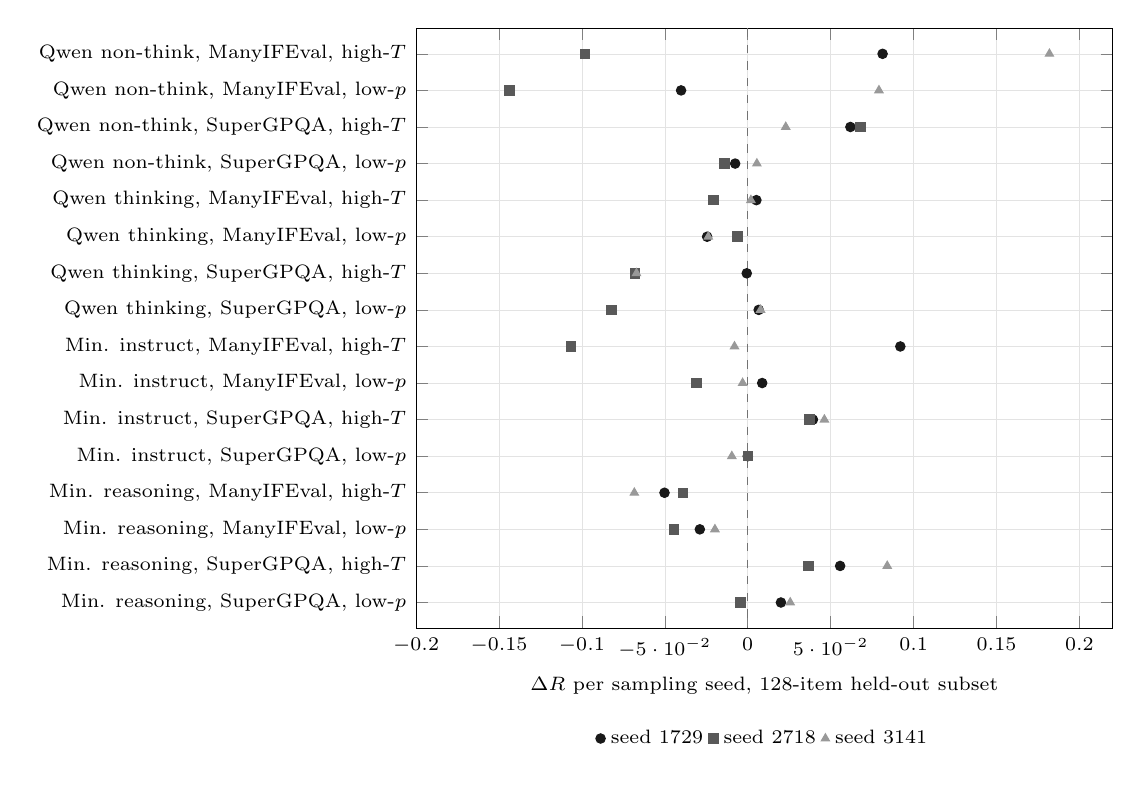
\begin{tikzpicture}
\begin{axis}[
  width=0.86\textwidth, height=9.2cm,
  ytick={0,1,2,3,4,5,6,7,8,9,10,11,12,13,14,15}, yticklabels={{Qwen non-think, ManyIFEval, high-$T$},{Qwen non-think, ManyIFEval, low-$p$},{Qwen non-think, SuperGPQA, high-$T$},{Qwen non-think, SuperGPQA, low-$p$},{Qwen thinking, ManyIFEval, high-$T$},{Qwen thinking, ManyIFEval, low-$p$},{Qwen thinking, SuperGPQA, high-$T$},{Qwen thinking, SuperGPQA, low-$p$},{Min. instruct, ManyIFEval, high-$T$},{Min. instruct, ManyIFEval, low-$p$},{Min. instruct, SuperGPQA, high-$T$},{Min. instruct, SuperGPQA, low-$p$},{Min. reasoning, ManyIFEval, high-$T$},{Min. reasoning, ManyIFEval, low-$p$},{Min. reasoning, SuperGPQA, high-$T$},{Min. reasoning, SuperGPQA, low-$p$}}, y dir=reverse,
  ymin=-0.7, ymax=15.7,
  xmin=-0.20, xmax=0.22,
  xlabel={$\Delta R$ per sampling seed, 128-item held-out subset},
  tick label style={font=\scriptsize}, label style={font=\scriptsize},
  legend style={font=\scriptsize, at={(0.5,-0.15)}, anchor=north, legend columns=3, draw=none},
  grid=major, grid style={gray!22,very thin}]
\draw[black!55,dashed] (axis cs:0,-0.7) -- (axis cs:0,15.7);
\addplot[only marks, mark=*, mark size=1.7pt, color=black!90] coordinates {(0.0813,0) (-0.0402,1) (0.0619,2) (-0.0076,3) (0.0052,4) (-0.0245,5) (-0.0006,6) (0.0066,7) (0.0920,8) (0.0087,9) (0.0393,10) (0.0000,11) (-0.0502,12) (-0.0289,13) (0.0557,14) (0.0200,15)};
\addlegendentry{seed 1729}
\addplot[only marks, mark=square*, mark size=1.7pt, color=black!65] coordinates {(-0.0982,0) (-0.1437,1) (0.0679,2) (-0.0139,3) (-0.0206,4) (-0.0063,5) (-0.0679,6) (-0.0821,7) (-0.1067,8) (-0.0310,9) (0.0371,10) (0.0000,11) (-0.0390,12) (-0.0446,13) (0.0366,14) (-0.0044,15)};
\addlegendentry{seed 2718}
\addplot[only marks, mark=triangle*, mark size=1.7pt, color=black!40] coordinates {(0.1819,0) (0.0791,1) (0.0229,2) (0.0055,3) (0.0019,4) (-0.0238,5) (-0.0671,6) (0.0077,7) (-0.0080,8) (-0.0031,9) (0.0462,10) (-0.0096,11) (-0.0684,12) (-0.0198,13) (0.0841,14) (0.0256,15)};
\addlegendentry{seed 3141}
\end{axis}
\end{tikzpicture}
